\hypertarget{test__match_8cpp}{}\subsection{test\+\_\+match.\+cpp File Reference}
\label{test__match_8cpp}\index{test\+\_\+match.\+cpp@{test\+\_\+match.\+cpp}}


An example of performing regex match against a pattern with J\+P\+C\+R\+E2 and getting the match count and match results.  


{\ttfamily \#include $<$iostream$>$}\newline
{\ttfamily \#include \char`\"{}jpcre2.\+hpp\char`\"{}}\newline
Include dependency graph for test\+\_\+match.\+cpp\+:\nopagebreak
\begin{figure}[H]
\begin{center}
\leavevmode
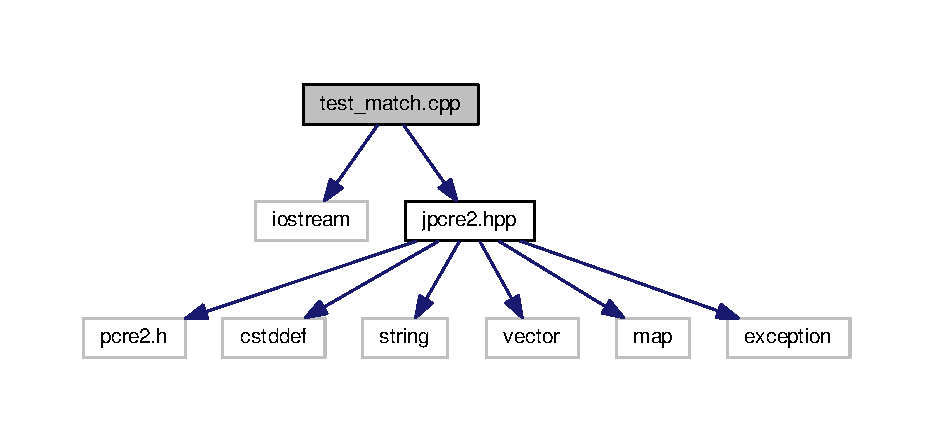
\includegraphics[width=350pt]{test__match_8cpp__incl}
\end{center}
\end{figure}


\subsubsection{Detailed Description}
An example of performing regex match against a pattern with J\+P\+C\+R\+E2 and getting the match count and match results. 

Shows how to iterate over the match results to get the captured groups/substrings. 
\begin{DoxyCodeInclude}

\textcolor{preprocessor}{#include <iostream>}
\textcolor{preprocessor}{#include "\hyperlink{jpcre2_8hpp}{jpcre2.hpp}"}


\textcolor{keywordtype}{int} main()\{

    \hyperlink{namespacejpcre2_ac1cf752c8fbb0be78020be3b80e77ce3}{jpcre2::VecNum} vec\_num0;   \textcolor{comment}{//Vector to store numbered substring Maps.}
    \hyperlink{namespacejpcre2_a2b121ae776ea5b2913839f418a7d856b}{jpcre2::VecNas} vec\_nas0;   \textcolor{comment}{//Vector to store named substring Maps.}
    \hyperlink{namespacejpcre2_a88a7aaf84cad627d34c8152e726168eb}{jpcre2::VecNtN} vec\_nn0;    \textcolor{comment}{//Vector to store Named substring to Number Maps.}
    
    \hyperlink{classjpcre2_1_1Regex}{jpcre2::Regex} re;          \textcolor{comment}{//It's not supposed to throw any exception.}
    
    \textcolor{comment}{//Compile the pattern}
    re.\hyperlink{classjpcre2_1_1Regex_a85d9a514ea86ae68533223adac6c6bd8_a85d9a514ea86ae68533223adac6c6bd8}{setPattern}(\textcolor{stringliteral}{"(?:(?<word>[?.#@:]+)|(?<word>\(\backslash\)\(\backslash\)w+))\(\backslash\)\(\backslash\)s*(?<digit>\(\backslash\)\(\backslash\)d+)"})  \textcolor{comment}{//set pattern}
          .\hyperlink{classjpcre2_1_1Regex_aed9865b58c60945e19f36fa310f5a595_aed9865b58c60945e19f36fa310f5a595}{setModifier}(\textcolor{stringliteral}{"mi"})                                                \textcolor{comment}{//set modifier}
          .\hyperlink{classjpcre2_1_1Regex_a03974fa7ba8f7c47186cb8d6f54934de_a03974fa7ba8f7c47186cb8d6f54934de}{addJpcre2Option}(\hyperlink{namespacejpcre2_a85c143271501e383843f45b9999c2f00_a85c143271501e383843f45b9999c2f00a5e8bab7c478015b19baf3e84ed00876e}{jpcre2::JIT\_COMPILE})                          
         \textcolor{comment}{//perform JIT compile}
          .\hyperlink{classjpcre2_1_1Regex_a2c7dcf12f26b2b046e147b013c8b5087_a2c7dcf12f26b2b046e147b013c8b5087}{addPcre2Option}(PCRE2\_DUPNAMES)                                                \textcolor{comment}{//
      add pcre2 option}
          .\hyperlink{classjpcre2_1_1Regex_aad1d5ef1e87f762f68a587eec4022e69_aad1d5ef1e87f762f68a587eec4022e69}{compile}();                                                       \textcolor{comment}{//Finally compile it.}
    
    std::cerr<<re.\hyperlink{classjpcre2_1_1Regex_a8606fff8b192c94f58ca9e82aa048c61_a8606fff8b192c94f58ca9e82aa048c61}{getErrorMessage}();
    
    \textcolor{comment}{// JIT error is a harmless error, it just means that an optimization failed.}
    
    \textcolor{comment}{//subject string}
    std::string subject = \textcolor{stringliteral}{"(I am a string with words and digits 45 and specials chars: ?.#@ 443 অ আ ক খ গ ঘ
        56)"};
    
    \textcolor{keywordtype}{size\_t} count = 0;
    
    count = re.\hyperlink{classjpcre2_1_1Regex_a519b0915bf1163c6ce6a4d674b30cfcd_a519b0915bf1163c6ce6a4d674b30cfcd}{initMatch}()                                      \textcolor{comment}{//Invoke the initMatch() function}
                  .\hyperlink{classjpcre2_1_1RegexMatch_a08c2e481fe8b9c001e67733fb4e33972_a08c2e481fe8b9c001e67733fb4e33972}{addModifier}(\textcolor{stringliteral}{"gf"})                           \textcolor{comment}{//set various parameters}
                  .\hyperlink{classjpcre2_1_1RegexMatch_a635c652195deaa8ebb9e107c4f972aab_a635c652195deaa8ebb9e107c4f972aab}{setSubject}(subject)                          \textcolor{comment}{//...}
                  .\hyperlink{classjpcre2_1_1RegexMatch_a2c7efe1ec2e13827f670db4ecedcd0a0_a2c7efe1ec2e13827f670db4ecedcd0a0}{setNumberedSubstringVector}(&vec\_num0)        \textcolor{comment}{//...}
                  .\hyperlink{classjpcre2_1_1RegexMatch_ae495431f57cae54363331237ab21b56c_ae495431f57cae54363331237ab21b56c}{setNamedSubstringVector}(&vec\_nas0)           \textcolor{comment}{//...}
                  .\hyperlink{classjpcre2_1_1RegexMatch_a04926e61d8b5f1d8bdf344efecd567d8_a04926e61d8b5f1d8bdf344efecd567d8}{setNameToNumberMapVector}(&vec\_nn0)           \textcolor{comment}{//...}
                  .\hyperlink{classjpcre2_1_1RegexMatch_aac4857cd8f5eae15b29b9afbe9023522_aac4857cd8f5eae15b29b9afbe9023522}{addPcre2Option}(0)                            \textcolor{comment}{//...}
                  .\hyperlink{classjpcre2_1_1RegexMatch_a5868aef3a146594ea1ebef34d122bb33_a5868aef3a146594ea1ebef34d122bb33}{match}();                                     \textcolor{comment}{//Finally perform the match}
    
    std::cerr<<\textcolor{stringliteral}{"\(\backslash\)n"}<<re.\hyperlink{classjpcre2_1_1Regex_a8606fff8b192c94f58ca9e82aa048c61_a8606fff8b192c94f58ca9e82aa048c61}{getErrorMessage}();
    std::cerr<<\textcolor{stringliteral}{"\(\backslash\)n"}<<re.\hyperlink{classjpcre2_1_1Regex_a1a639ae4090b88609c03e9268faf02d8_a1a639ae4090b88609c03e9268faf02d8}{getWarningMessage}(); \textcolor{comment}{//Invalid modifier: f}
    
    
    \textcolor{comment}{// re.reset(); // re-initialize re}
    
    
    std::cout<<\textcolor{stringliteral}{"\(\backslash\)nTotal number of mathces: "}<<count<<std::endl;
    \textcolor{comment}{//Now let's access the matched data}
    
    \textcolor{comment}{//Each of these vectors contains maps.}
    \textcolor{comment}{//Each element in the vector specifies a particular match}
    \textcolor{comment}{//First match is the vector element 0, second is at index 1 and so forth}
    \textcolor{comment}{//A map for a vector element, i.e for a match contains all of its substrings/capture groups}
    \textcolor{comment}{//The first element of the map is capture group 0 i.e total match}
    
    
    \textcolor{keywordflow}{for}(\textcolor{keywordtype}{size\_t} i=0;i<vec\_num0.size();++i)\{
        
        
        std::cout<< \textcolor{stringliteral}{"\(\backslash\)n################## Match no: "}<<i+1<<\textcolor{stringliteral}{" ####################\(\backslash\)n"};
        
        
        
        \textcolor{comment}{//This vector contains maps with number as the key and the corresponding substring as the value}
        std::cout<<\textcolor{stringliteral}{"\(\backslash\)n-------------------------------------------------------------------------"};
        std::cout<< \textcolor{stringliteral}{"\(\backslash\)n--- Numbered Substrings (number: substring) for match "}<<i+1<<\textcolor{stringliteral}{" ---\(\backslash\)n"};
        \textcolor{keywordflow}{for}(jpcre2::MapNum::iterator ent=vec\_num0[i].begin();ent!=vec\_num0[i].end();++ent)\{
            std::cout<<\textcolor{stringliteral}{"\(\backslash\)n\(\backslash\)t"}<<ent->first<<\textcolor{stringliteral}{": "}<<ent->second<<\textcolor{stringliteral}{"\(\backslash\)n"};
        \}
        
        
        
        \textcolor{comment}{//This vector contains maps with name as the key and the corresponding substring as the value}
        std::cout<<\textcolor{stringliteral}{"\(\backslash\)n-------------------------------------------------------------------------"};
        std::cout<< \textcolor{stringliteral}{"\(\backslash\)n--- Named Substrings (name: substring) for match "}<<i+1<<\textcolor{stringliteral}{" ---\(\backslash\)n"};
        \textcolor{keywordflow}{for}(jpcre2::MapNas::iterator ent=vec\_nas0[i].begin();ent!=vec\_nas0[i].end();++ent)\{
            std::cout<<\textcolor{stringliteral}{"\(\backslash\)n\(\backslash\)t"}<<ent->first<<\textcolor{stringliteral}{": "}<<ent->second<<\textcolor{stringliteral}{"\(\backslash\)n"};
        \}
        
        
        
        \textcolor{comment}{//This vector contains maps with name as the key and number as the value}
        \textcolor{comment}{//i.e the number (of substring) can be accessed with the name for named substring.}
        std::cout<<\textcolor{stringliteral}{"\(\backslash\)n-------------------------------------------------------------------------"};
        std::cout<< \textcolor{stringliteral}{"\(\backslash\)n--- Name to number mapping (name: number/position) for match "}<<i+1<<\textcolor{stringliteral}{" ---\(\backslash\)n"};
        \textcolor{keywordflow}{for}(jpcre2::MapNtN::iterator ent=vec\_nn0[i].begin();ent!=vec\_nn0[i].end();++ent)\{
            std::cout<<\textcolor{stringliteral}{"\(\backslash\)n\(\backslash\)t"}<<ent->first<<\textcolor{stringliteral}{": "}<<ent->second<<\textcolor{stringliteral}{"\(\backslash\)n"};
        \}
    \}
    \textcolor{keywordflow}{return} 0;
\}
\end{DoxyCodeInclude}
 \begin{DoxyAuthor}{Author}
\href{https://github.com/neurobin}{\tt Md Jahidul Hamid} 
\end{DoxyAuthor}
